\section{System Design and Architecture}
In this section, we describe \system{}, a prototype feature store designed to support flexible, user-defined prioritization and load shedding policies for efficiently maintaining feature tables derived from streaming data. 

\system{} follows the design of existing modern streaming systems: inputs are streamed through a series of operators  (e.g. map, join, window) expressed as a DAG through which features are computed.  There are two primary differences: 1.) operators support user-defined prioritization policies which can be configured by per-key parameters generated by the scheduler, 2.) feature maintenance policy parameters are determined by approximating feature store loss from prior query and event traces using an \textit{offline planner}. These properties allow \system{} to adapt its policy configuration to improve feature store loss, and adopt more flexible policies for prioritizing events as compared to standard streaming systems. 

\label{s:design}
\natacha{It'd be nice to have an overview of what you're going to talk about and even an architecture design "intro". At this point, I'm still unsure what \system{} is}
\subsection{API}
\label{ss:design:api}
%

%Data sources are defined in terms of \textit{source tables}, which can be transformed into downstream feature tables. Feature tables can be queried by downstream applications by being marked as queryable, e.g. line 5 in \cref{lst:api}. We showcase \system{}'s featurization API in \cref{lst:api}, which implements a time series decomposition pipeline.
%
%Each feature operator maintains a corresponding \textit{feature table},
%which is generated from the operator's parent tables and
%stores the operator's outputs\natacha{What are the operator's parent tables? %Given we go straight from scheduling to System design}.
%
%To enable the sharing of features across applications, feature tables can be made
%externally queryable via a HTTP interface.
% Each feature operator is responsible for maintaining a \textit{feature table},
% which can be made externally queryable.
%
% Each feature table is defined in terms of a single parent table for map and window operators,
% or two parent tables for the join operator.
%
% By constructing featurization pipelines as a DAG of operators, \system{} maintains a clear
% lineage of feature tables, so queried feature keys can be traced back to up.
\natacha{What's the link between shared computation and what we were talking above. Is this a new design? Is is standard feature store architecture??}
%
% \system{} encourages users to define feature as function of other features,
% to define clear dependencies between multiple feature tables and encourage shared computation.
%
%We showcase \system{}'s featurization API in \cref{lst:api}, which implements a time series decomposition pipeline. 
%

%

%


% Each feature table can optimally include a \textit{load shedding policy} and \textit{prioritization policy} for processing parent table updates. The prioritization and load shedding policies can be adjusted by policy parameters (such as by changing the set of prioritized keys, or the sampling rate of events). We show an example of a prioritization policy for implementing LIFO prioritization in \cref{lst:prioritization}, and an example of random sub-sampling load shedding in \cref{lst:shedding}.

\begin{figure}[t]
    \begin{lstlisting}[
language=Python, 
caption=Defining a maintained feature table of user embeddings with RALF. , 
escapechar={|},  
basicstyle=\small,
commentstyle=\color{blue}\sffamily,
stringstyle=\color{red}\sffamily,
numberstyle=\color{gray}\sffamily,
label={lst:api}
]
# Source table 
source = ralf.tables.kafka_source(topic="user_data")

# Queryable feature table 
embedding = source
    .map(UserEmbeddingModel, model_file="model.pt")
    .as_queryable("user_features")
    .set_replicas(4)
    .set_default_error(0.01)
\end{lstlisting}

 
    \begin{lstlisting}[language=Python, caption=Event load shedding example using scheduling parameters., escapechar={|}, label={lst:shedding}]
def random_subsample(record: Record): 
    return random.random() < /
        |\color{purple}policy\_params|["sample_rate"][record.key]
\end{lstlisting}
    \begin{lstlisting}[language=Python, caption=Event prioritization example implementing LIFO prioritization., label={lst:prioritization}]
def lifo_prioritization(
    current: Record, candidate: Record):
    return (current.processing_time
             > candidate.processing_time)
\end{lstlisting}
\end{figure}


%
%\subsection{Operators for Featurization}
%\label{ss:design:operators}
%
\natacha{What you're describing here doesn't seem to be an an API, but a design?}
\system{}'s API defines featurization pipelines in terms of a DAG of \textit{feature tables}, where each feature table is defined in terms of terms of an operator and one or more input (i.e. parent) feature tables. Feature tables can be make externally queryable through an HTTP interface, and are incrementally updated as new data is streamed into the pipeline. We show an example definition of a feature table in Listing \cref{lst:api}.
%Similar to streaming dataflow systems, \system{} consists of a set of operators chained into a DAG.
%
%As opposed to streams, \system{} uses operators to define feature tables which may be queried.
\peter{May need to elaborate on how \system{} is different.}
\kevin{+1 to this, and also to the operators}
\natacha{You had an almost identifcal first sentence in 4.1 (and you already discussed operators there)}
%

\system{} provides a general-purpose API for constructing operators, as well as reference implementations
for source, map, window, streaming join, and sink operators.
\natacha{Now you're talking about an API, but API was supposed to be 4.1. Could we "merge" 5.1 and 4.2? I can't really tell the difference between the two. }
%
\system{} innovates on the window and map operator implementations with built-in mechanisms that enable update scheduling to account for resource cost and downstream error. 
%

% Architecturally, \system{} resembles a streaming dataflow system. Users define source, map, window, and sink operators. These operators are chained into a DAG. 

\myparagraph{Sources and Sinks}
%
\system{} contains abstractions for building \textit{source operators}, which ingest data
from external sources, and
\textit{sink operators}, which emit data to external systems.
%
Reference source operator implementations read data from files, Kafka Streams~\cite{kafka},
and Redis streams~\cite{redis-streams}.
%
\system{} also provides sink operator implementations for saving data to files and Redis~\cite{redis}.
\peter{Please add more reference source and sink implementations if \system{} provides them.}


%
\myparagraph{Maps and Joins}
%
\system{} provides reference implementations of map and join operators,
which run expensive, bottleneck feature functions.
%
Map operators may be used to apply transformations to single or windowed updates. Join operators are similar to Map operators, but allow for multiple input (i.g. parent) tables. 
%
%Join operators may be used to generate complex features
%derived from multiple sources, and can generate predictions
%by running a model using stored weights joined with data.
%
%\sarah{maybe just frame joins as maps that can take multiple inputs?}
%\system{}'s map and join operators implement mechanisms for intelligently allocating resources for feature computation.
%
To manage the high cost of computing features, Map and Join operators may include user-define policies for event prioritization and load shedding. Users can implement \textit{per-key prioritization} policies to prioritize events for a single key, or \textit{cross-key prioritization} policies to prioritize across keys. These policies can take in \textit{policy parameters} as inputs to configure feature maintenance. We show examples of event prioritization and event load shedding policies in \cref{lst:prioritization} and \cref{lst:shedding}, respectively. 

% \cref{ss:design:scheduler}.
% \natacha{May include? Are you talking about your system or feature operators in general? I would say "include". I would also say "Feature operators in \system{}?"}
% %
% Each feature table can also define policies for event prioritization and load shedding. These policies can take in \textit{policy parameters} as inputs to configure the policy. We show examples of event prioritization and event load shedding policies in \cref{lst:api} and \cref{lst:api}, respectively. 

%
% As shown in \cref{fig:arch}, maps and joins may use prioritization policies
% (further discussed in \cref{ss:design:scheduler})
% to re-order processing in order to prioritize the featurization of critical keys and updates.
%

\myparagraph{Windowing}
\system{} provides an additional mechanism to control feature updates through \textit{dynamic windowing}, which allow per-key window sizes and window slide sizes.
%
%While traditional window operators only allow a static configuration across streams,
%\system{}'s window operator supports per-key configuration at runtime.
%\peter{I'm not sure if this claim is true, e.g. windowing in SQL using another table to set window size.Also, different window configurations per key might be possible when grouping by key.}
%
% enable \system{} to intelligently balance compute cost and feature accuracy.
%
Window operators can manage compute costs by increasing window size in order to process data in larger batches,
and by changing the window slide size to change the rate at which data is emitted to control the rate of feature updates per-key.
%
% For example, a featurization pipeline which detects anomalies across a rapidly-changing time series
% (\cref{ss:evaluation:time-series-decomposition}) benefits more
% from a smaller window slide size compared to a stable time series.
% \peter{Consider adding a small experiment to elaborate on/quantify this}
% \sarah{Maybe we could improve figure 2 and reference it here, since it's showing how some time series in the yahoo dataset need very few re-fits}
% %
% The smaller slide size generates more frequent updates, which enables the rapid detection of anomalous changes
% in the time series by downstream operators.
% %
% On the other hand, generating more updates results in more work for downstream operators which may
% run expensive anomaly detection models.
% %
% Because time series for different keys may change at different rates, \system{}'s window operator will
% re-configure each key's window configuration in order to find the ideal trade-off between cost
% and delay in anomaly detection by optimizing the latency-aware feature store accuracy.
% \natacha{This paragraph feels a little strange as it sounds like you didn't have Section 3, and you don't talk about Section 3 at all here. Presumably, isn't the reason why you support per-key window configuration a response to the "findings" you made in Section 3? }
%
% Thus, dynamically adjusting per-key window slide size at runtime can balance compute costs for
% timely anomaly detection by optimizing the latency-aware feature store accuracy.
%

%

%

%\system{} innovates on both the window operator and map operator. 

% \myparagraph{Window Operators}  While traditional windowing operator only allow setting a fixed sized window for the entire stream, \system{}'s windowing operator allow per-key window configuration. For example, in the anomaly detection model use case \kevin{explain earlier what this is}, a time series that's rapidly changing would benefit more from smaller sliding size for a sliding window operator as compare to a very stable time series. For rapidly changing time series, maybe we should emits the sliding window every 2 records to capture any recent changes; while for a stable time series, we can just emits a sliding window every 128 records \kevin{is this very application specific?}. The smaller the slide size, the more records that the downstream operators need to process, therefore increase the compute cost; but smaller the slide size also means we will be capture the freshest data in downstream operators and drive up accuracy. Therefore, *per-key window configuration* allows \system{} to balance compute cost and feature accuracy intelligently. This feature can be implemented as custom windowing operator in traditional streaming dataflow system, however \system{} made it built in and as a first class primitive.
% \sarah{this per-key thing applies to all operator scheduling parameters though, right?}

\subsection{Scheduling Updates}
\label{ss:design:scheduler}
%
\system{} contains a multi-level scheduler which determines policy parameters (\cref{s:policy-parameters}) to configure update processing. 
The scheduler contains an offline planner which generates feature maintenance policy parameters, and performs cross-key and event prioritization at the operator level. 

\natacha{This is where I'm starting to see the "link". One thing I'm curious about though is that you talked about how the load shedding/priority policies were defined per operator (which made it sound local and user defined), but now you're talking about a global scheduler}
\sarah{make this focux on operator level scheduling - assume only one layer is bottleneck for now}
\system{} provides mechanisms for adjusting policy parameters at runtime (e.g., changing the per-key priority, or the sampling rate of updates), enabling featurization pipelines to respond to changes in incoming data without a reduction in featurization loss.



%



%
% The global feature-prioritization scheduler uses the chooses high-value updates to deliver to operators
% for processing, and may prioritize certain keys and features that are critical to 
% application performance.
% \peter{Feature-prioritization scheduler is a mouthful and sounds gimmicky.
% Consider changing name to something else.}
%
% The local operator-level scheduler uses the prioritization and load-shedding policies
% to ensure high-value updates are processed quickly and to manage load.
% \peter{\cref{fig:arch} needs more info about global scheduling, or we need another diagram.}
%
% \system{} has a built in multi-level scheduler into each map operator. The scheduler utilize contextual information about the feature, incoming events, and global accuracy scores to prioritize events among all the keys. 
% The scheduler has three part: (1) per-key priority queue (2) eviction process (3) cross-key load balancer. These three components enables the operator to become feature quality aware and explicitly prioritize more valuable events over the other. This feature is not present in traditional streaming dataflow system because it is built to process data in FIFO (first-in, first out) ordering.
%


%
% We present an example LIFO priorization policy in \cref{lst:prioritization}, and
% and random sub-sampling load shedding policy in \cref{lst:shedding}.
\peter{TODO: should showcase an adjustable policy instead.}
\natacha{The link between this part and Section 3 is not obvious. How should I think of the relationship between them?}

\subsubsection{Offline Planner}
\label{s:planner}
The offline planner runs simulations to select feature maintenance policy parameters to improve downstream performance metrics under resource constraints.  

\system{} uses a discrete time simulator to generate execution plans for various policy configurations. Each \system{} operator is implemented in our simulator, where map and join operators support user-define prioritization policies. The simulator processes samples recent event and query traces to evaluate downstream accuracy and resource cost metrics for different per-key policy configurations. To optimize the feature maintenance policies across keys, \system{} use a mixed integer numeric optimizer (OR-tools \cite{van2014or}) to find the ideal per-key parameters. The linear program is written to solve for the lowest cost combination of feature policy per key, under a compute budget constraint. 


% The simulator supplies an offline batch-optimized version of the pipeline with sampled data to initialize features, and recreates query patterns using stored traces.
% \peter{Maybe slightly overclaiming}
% \natacha{Emphasise that this is a lot cheaper because batch? Otherwise it's odd that to save cost, we have to "simulate" in full}

% %
% \subsubsection{Offline Planner}
% %

% To ensure that \system{} maintains a high accuracy,
% an offline planner periodically proposes and evaluates several plans
% (i.e. configurations of operators). 
% \peter{I'm using low feature store loss/high accuracy interchangeably.
% We need to clarify that they mean the same thing in section 3,
% or choose 1 term.}
% \natacha{query plan or scheduling policy? I'm pretty sure you're talking about scheduling policy (and when you say reconfiguring operators, you're talking about window size, etc) but the way that you write it initially makes it sound like you're talking about  query plans and join ordering etc.}
% %
% \system{} selects the highest-scoring plan, and reconfigures its operators
% at runtime to dynamically improve how features are computed.
% %

% %
% % To score plans, \system{} uses a discrete event simulator which uses
% % the application-level accuracy metric to evaluate plans on
% % samples of live production data.
% % \peter{How are plans proposed?}
% %

% %
% For each plan and key, the planner tracks the resource costs of featurization, and
% computes a score by summing the losses of all queries for that key's features.
% %
% As a result, each plan's per-key score is weighted its importance in terms of number
% of queries.
% %
% \system{} selects a plan by running a constraint optimization solver over the set of
% per-plan scores and costs in order to generate the highest scoring plan
% which meets the user-specified resource constraints.
% \peter{This text is rough}
% \peter{Need to add in that the cost of planning is amortized since it runs at a low frequency}
% %

%
% \subsubsection{Feature Prioritization}
% \label{ss:design:feature-prioritization}
% %
% The feature-prioritization scheduler is responsible for ensuring that high-value
% events are quickly processed by controlling how updates are released to operators.
% %
% This scheduler acts as an accuracy-aware load balancer, and releases updates
% to operators to ensure smooth operatation of the system
% (e.g., by delaying updates to avoid excess load)
% in a way that minimizes the impact on accuracy.
% %
% The scheduler is implemented as a priority queue, and uses a fast heuristic
% to score updates.
% %
% \system{}-provided policies include LIFO which prioritizes new updates,
% round-robin which ensures cross-key fairness, as well
% as more advanced strategies to prioritize certain keys.
% \peter{We need to elaborate on the more advanced strategies.}
% %

%
\subsubsection{Online Scheduling}
\label{ss:design:operator-level-scheduler}
%
\system{}'s feature maintenance policies work on on the operator level, and implement prioritization both across keys and within each per-key event queue.  
%
Each operator contains both a cross-key queue for cross-key prioritization, and a per-key queue for event prioritization and eviction. 
% Each key contains a priority queue of updates, which are scored using a similar \sarah{this is inconsistent with the diagram}
% heuristic as in \cref{ss:design:feature-prioritization} (e.g., LIFO).
% %
% Unlike \cref{ss:design:feature-prioritization}, the operator-level scheduler
% also contains an eviction policy, which can discard unimportant or stale updates.
% %
The eviction policy has two opportunities to discard an update:
1.) before insertion into the priority queue, enabling
commonly-used uniform sampling strategies, and
2.) after removal from the queue, enabling the operator
to skip updates that are only important for a short amount of
time and have gone stale.
%
The parameters determined by the offline planner configure how keys and events are prioritized and processed. 
%
\peter{Need to iterate on this subsection to clarify things,
and improve the motivation and intuition behind the simulator and
multi-level scheduler.}


% In order to evaluate the scheduling policy for prioritizing events and keys, \system{} utilize discrete event simulator to test policies on sample of live production data. Additionally algorithm and plan selection can be performed offline. For example, in the time series prediction workload, we used offline simulator to simulator different selection of window sizes; then run through a constraint optimization solver to optimize accuracy. 
% The offline simulator generates traffic patterns and run through the model in offline batch processing mode. Concretely, its input is sample traffic traces, configuration to test, and model runtime. Optionally, one can run the records through the actor model both within the simulation process or outside of the simulation process to access the end to end accuracy. 
% We think the offline planning component is critical to \system{}. It should be a companion to continuously fine-tune the \system{} online streaming data processing pipeline given workload changes. In the future, \system{} can even adjust the plan on-the-fly without explicitly reconfiguration, when utilizing the offline simulator.
% The offline component provides a feedback mechanism to propagate configuration changes in respond to traffic and  events pattern changing overtime, with the final goal of continuously optimizing end to end feature accuracy.
% 
% %
% \subsubsection{Prioritization Mechanisms}
% %
% \myparagraph{Local: Event Prioritization}
% The first level scheduling is done on a per-key basis. Each key has a priority queue where events corresponding to that key is sorted into. For example, for time series anomaly detection pipeline , latest events are always prioritized over previous ones; for wikipedia edits process, edits with more content in them can sometimes be more useful than a simple typo change. 
% 
% Eviction is performed both before event insertion into the priority and before event being picked from the priority queue. The first allows implementing a uniform sampling strategy that's common in baseline featurization system. The latter allow us to skip the map if the current events no longer matters. 
% 
% \myparagraph{Global: Key Prioritization}
% The cross-key load balancing is performed as the second level scheduling. Its responsibility is to pick the most value events among the keys to deliver to the actual map processing operator. By default it can round-robin among all the keys. It can also pick the key with latest or oldest timestamped events at the top of their queue. Additionally, \system{} implemented more advanced strategy to prioritize certain keys over the others. 



% \begin{figure}[t]
% \begin{center}
% 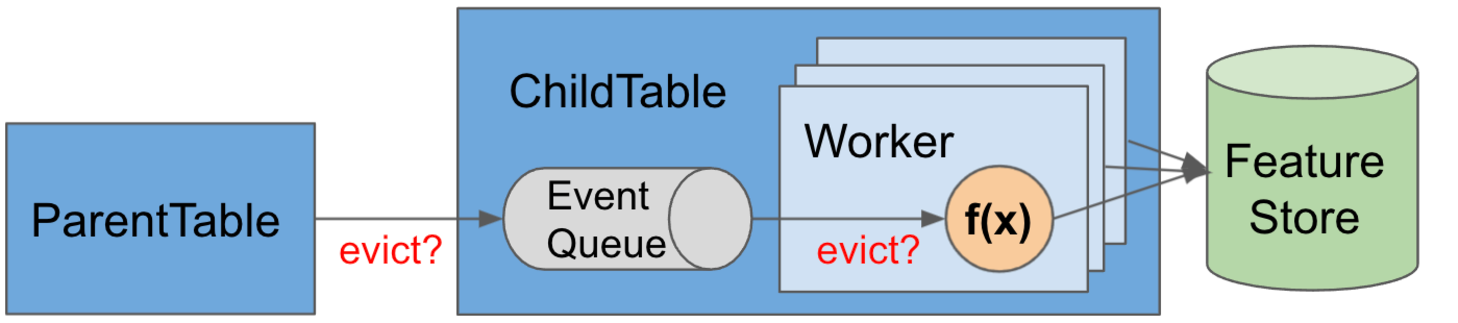
\includegraphics[width=8cm]{ralf/figures/architecture3.pdf}
% \centering
% \end{center}
% \caption{\label{fig:arch} \system{} System Architecture }\label{f:arch}
% \end{figure}

%
\subsection{Implementation}
\label{ss:design:implementation}
%
\jmh{It's a missed opportunity not to do this in a DBMS with UDFs like Postgres, and talk about materialized views. If you had done so, you'd have a very VLDB-friendly exposition of the APIs, clean example code, clear view materialization opportunities, etc.}
%
We emphasize that \system{} is a set of ideas for accuracy-aware featurization, and
can be implemented on several systems.
%
We construct a full prototype of \system{} in about 1,500 lines of Python code.
%
Our prototype is built atop Ray~\cite{ray}, because many
popular featurization and machine learning libraries (e.g., Tensorflow~\cite{tensorflow})
use Python, and Ray is designed to support machine learning workloads.
%
% To show the generality of our contributions, we also provide a reference implementation
% in Timely Dataflow~\cite{timely-dataflow-book}.
%
%
%\myparagraph{Ray prototype}
%
\system{} runs atop Ray's actor framework.
%
Each operator is implemented as a pool of Ray actors, in which each
individual actor manages a subset of keys.
%
Because operators are sharded across a pool of actors, \system{} can easily
scale out the operator to improve processing throughput.
%
Updates are exchanged by calling methods on Ray actors belonging to other operators.
%
Under the hood, Ray serializes and ships the updates via RPC.
%
Upon receiving an update, the operator-level scheduler
(\cref{ss:design:operator-level-scheduler})
the invokes eviction and prioritization policies, and then inserts the update
into a priority queue.
%
A set of runner threads poll the priority queue and process updates.
%
% To avoid starvation due to Python's global interpreter lock, operators
% are implemented using Python's asyncio interface.
%
% In addition, the Ray prototype benefits from featurization and machine learning
% libraries that are backed by compiled languages as they release the
% global interpreter lock when perfoming expensive computations.
%

%
% \myparagraph{Timely Dataflow prototype}
% %
% The Timely prototype is developed as a library of \system{} operators,
% which consist of $500$ lines of Rust code.
% %
% \system{} operators extend Timely's existing operator interfaces,
% and take advantage of Timely's data-parallel architecture to scale out.
% %
% While Timely-based featurization pipelines are written in Rust,
% the library provides custom operators which support calling Python
% code from Rust.
% %
% \peter{TODO: discuss eventually consistent joins}
% \peter{TODO: discuss prioritization in Timely}

\jmh{To me the only value of the multiple implementations is to convince the skeptical systems reader that you've solved the problem in a portable way. See my comment below in related work. I wouldn't dwell on evaluating Ray vs Timely vs Noria. Phooey. Now, if one of them lacks the expressivity you need to do the right thing, DO bring that up here, but don't run an evaluation to establish an expressivity problem. By contrast, if one of them is more efficient---e.g., provides a faster update rate---is that really pertinent to your contribution of reframing the feature store freshness problem? Or is it just kind of "System X is more efficient at the class of queries you see here than System Y", but it's not fundamental -- these queries could be tuned up in System Y orthogonal to our techniques. I care more about you characterizing that class -- and then letting the systems optimize for it later if they choose. Finally, there are many systems here you're not evaluating that can express this stuff---notably many database engines---which makes this feel to me like pandering to a narrow audience and its myopia. In the real world I might want to use Snowflake or a high-performance main-memory database; I'm probably not gonna use Noria or Timely. Independent of these pragmatics, why does this paper care anyhow? I feel like you're soiling your beautiful big idea of ``it's the application metric that matters, stupid''  with other people's obsession with system internals of research prototypes. (Grumpy database guy signing off!)}

% \system{} is a set of ideas that bring ML feature quality awareness into streaming dataflow system. It it agnostic to any underlying systems. For this paper, we implemented a prototype system on Ray and a comparison system on Timely Dataflow. We chose to implemented on Ray because it's easy to integrate Python based featurization pipeline and machine learning libraries into the streaming pipeline.
% 
% For the Ray prototype implementation, each operator runs on Ray Actors. Each operator can be sharded by record key. Sharding makes it easy to horizontally scale out the processing throughput. We then use Ray's actor call as RPC mechanism to send records among the operators. 
%
% For the timely dataflow implementation,

% \myparagraph{Offline planner}
% The offline planner was built using an off-the-shelf discreate event simulation library, simpy \cite{matloff2008introduction}. We use the simulation library to generate traces with samples of production workload and compute its accuracy score. To optimize the featurization policies across keys, we use a mixed integer linear program solver (OR-tools \cite{van2014or}) to optimize the final feature policies. The linear program is written to solve for the lowest cost combination of feature policy per key, under a compute budget constraint.
